\documentclass{beamer}

%%%% Packages
\usepackage{amsmath, amsthm, amssymb}
%% \usepackage[english]{babel}
\usepackage{array}              % for >{} in table column
% specification
\usepackage{color}              % for color definition
\usepackage{colortbl}
\usepackage{graphicx}
\usepackage{multirow}           % for multirow
\usepackage{multicol}           % for multiple columns
\usepackage{tabularx}           % for centering in table
\usepackage{tikz}               % for drawing diagrams
\usetikzlibrary{arrows,graphs,positioning,shapes}

%%%% Macros and Definitions
\definecolor{firebrick4}{RGB}{139,026,026}
\definecolor{gray12}{RGB}{31,31,31}
\definecolor{gray24}{RGB}{61,61,61}
\definecolor{gray57}{RGB}{145,145,145}
\definecolor{gray71}{RGB}{181,181,181}
\definecolor{gray84}{RGB}{212,212,212}
\definecolor{lightcyan4}{RGB}{122,139,139}
\definecolor{dodgerblue4}{RGB}{16,78,139}
\definecolor{dodgerblue3}{RGB}{24,116,205}

\newcommand{\indentpar}[1]{{\setlength{\parindent}{1cm} #1}}
\newcommand{\visiblealert}[2]{\visible<#1->{\alert<#1->{#2}}}
\DeclareMathOperator*{\argmax}{arg\,max}

% TIKZ setup for drawing graphs
% \pgfkeysalso doesn't change the path
\tikzset{onslide/.code args={<#1>#2}{ \only<#1>{\pgfkeysalso{#2}} }}

\tikzset{temporal/.code args={<#1>#2#3#4}{
    \temporal<#1>{\pgfkeysalso{#2}}{\pgfkeysalso{#3}}{\pgfkeysalso{#4}}
}}

\tikzset{fontscale/.style = {font=\relsize{#1}}
    }

\tikzstyle{highlight}=[red,ultra thick]

%%%% Presentation Setup
\mode<presentation>
    {
      \usetheme{Ilmenau}
      \usecolortheme{beaver}
      \usefonttheme[onlylarge]{structuresmallcapsserif}
    }
    \setbeamercolor{title}{fg=dodgerblue4}
    \setbeamercolor{frametitle}{fg=dodgerblue4}
    \setbeamercolor*{palette secondary}{fg=dodgerblue4,bg=gray84}
    \setbeamercolor*{palette tertiary}{fg=white,bg=dodgerblue4}
    \setbeamercolor*{item}{fg=dodgerblue4}
    \setbeamercolor*{block title example}{bg=gray24,fg=white}

    \setbeamerfont{author}{size=\scriptsize}
    \setbeamerfont{institute}{size=\scriptsize}
    \setbeamerfont{date}{size=\tiny}
    \setbeamerfont{normal text}{size=\scriptsize}

    \beamertemplatenavigationsymbolsempty

    %%%% Title
    \title[PhD Report 2014]{PhD Report -- December 2014}
    \author[Sidorenko]{Wladimir Sidorenko\\ \texttt{uladzimir.sidarenka{@}uni-potsdam.de}}
    \institute[Uni Potsdam]{University of Potsdam}
    \date{\today}

    \pgfdeclareimage[interpolate=true,height=2.5cm]{logo}{img/uni_potsdam_logo.png}
    \titlegraphic{\pgfuseimage{logo}}

    %%%% Document
    \begin{document}
    %%%%%%%%%%%%%%%%%%%%%%%%%%%%%%%%%%%%%%%%%%%%%%%%%%%%%%%%%%%%%%%%%%
    %%% Title Page
    \begin{frame}{}
      \titlepage
    \end{frame}

    %%%%%%%%%%%%%%%%%%%%%%%%%%%%%%%%%%%%%%%%%%%%%%%%%%%%%%%%%%%%%%%%%%
    %%% Table of Contents
    \begin{frame}{Contents}
      \tableofcontents
    \end{frame}

    %%%%%%%%%%%%%%%%%%%%%%%%%%%%%%%%%%%%%%%%%%%%%%%%%%%%%%%%%%%%%%%%%%
    %%% Previous Work
    \section{Previous Work}
    \subsection{Corpus}
    \begin{frame}{\insertsubsection}
      Manually annotated sentiment corpus consisting of 3996 Twitter
      messages drawn from four different topics based on three
      disjoint formal criteria.
    \end{frame}

    \subsection{Classification Results}
    \begin{frame}{\insertsubsection}
      \begin{table}
        \tiny
        \caption{\scriptsize Classification results for automatic sentiment
          analysis.}  \centering
        \begin{tabular}{p{0.25\textwidth}*{3}{>{\centering\arraybackslash}p{0.15\textwidth}}}
          \hline\noalign{\smallskip}
          Classification Element & Precision & Recall & F-Measure\\\hline
          \multicolumn{4}{c}{\cellcolor{lightcyan4}Training Set}\\
          Sentiment & 99.23 & 85.86 & 92.06\\
          Source & 91.74 & 73.36 & 81.53\\
          Target & 96.24 & 74.88 & 84.23\\
          \hline\multicolumn{4}{c}{\cellcolor{lightcyan4}Test Set}\\
          Sentiment & 24.26 & 16.79 & 19.85\\
          Source & 50 & 28.12 & 36\\
          Target & 29.73 & 17.32 & 21.89\\
          \noalign{\smallskip} \hline
        \end{tabular}
      \end{table}
    \end{frame}

    %%%%%%%%%%%%%%%%%%%%%%%%%%%%%%%%%%%%%%%%%%%%%%%%%%%%%%%%%%%%%%%%%%
    %%% On-going Work
    \section{On-going Work}
    \begin{frame}{\insertsection}
      Ways to improve the performance:
      \begin{itemize}
      \item Change model;
      \item Change features;
      \item Change data.
      \end{itemize}
    \end{frame}

    \subsection{Model Change}
    \begin{frame}
      \frametitle{\insertsubsection}
      \tiny
      \vspace*{\fill}
      \begin{minipage}[t]{0.5\linewidth}
        \begin{center}
          \tikzset{mynode1/.style={}}
          \tikzset{mynode2/.style={}}
          \tikzset{mynode3/.style={}}
          \tikzset{mynode4/.style={}}
          \tikzset{mynode5/.style={}}
          \only<4->{\tikzset{mynode1/.style={text=white,fill=dodgerblue4}}}
          \only<5>{\tikzset{mynode2/.style={text=white,fill=dodgerblue4}}}
          \only<6>{\tikzset{mynode3/.style={text=white,fill=dodgerblue4}}}
          \only<7>{\tikzset{mynode4/.style={text=white,fill=dodgerblue4}}}
          \only<8>{\tikzset{mynode5/.style={text=white,fill=dodgerblue4}}}

          \begin{tikzpicture}
            [auto=left,scale=0.6,
              every node/.style={rectangle,draw,font=\tiny,fill=gray84,minimum size=15pt},
              word/.style={draw=none,fill=none},
            ]

            \matrix[ampersand replacement=\&,fill=none,draw=none,rectangle,row sep=0.1cm,%
              column sep=0.8cm] {
              \node[mynode5]{SRC}; \& \node{SRC}; \& \node{SRC}; \& \node{SRC};\\
              \node[mynode4](n31){TRG}; \& \node{TRG}; \& \node{TRG}; \& \node{TRG};\\
              \node[mynode3](n21){STM}; \& \node[mynode1](n22){STM}; \& \node{STM}; \& \node{STM};\\
              \node[mynode2]{NON}; \& \node{NON}; \& \node{NON}; \& \node{NON};\\
              \node[word]{Ich}; \& \node[word]{mag}; \& \node[word]{diesen}; \& \node[word]{Politiker};\\
            };
            %% \draw (n21) -- (n22);\\
            %% \draw (n31) -- (n22);\\
          \end{tikzpicture}
        \end{center}
      \end{minipage}
      \begin{minipage}[t]{0.48\linewidth}
        \begin{center}
          \vspace*{\fill}
          \only<1>{
            \raggedright{\: Unnormalized probability of the tag sequence:}
            \begin{equation}
              \tilde{P}(X,Y) = exp\Big\{\sum_i{\Theta_{i} * f_{i}(x = X, y = Y)}\Big\}
            \end{equation}

            \raggedright{\: Normalized probability of the tag sequence:}
            \begin{equation}
              P(Y|X) = \frac{\tilde{P}(X,Y)}{\sum_{Y}\tilde{P}(X,Y)}
            \end{equation}
            \pause
          }

          \only<2>{
            \raggedright{\: Dataset:}
            \begin{equation*}
              \mathcal{D} = \{x[m],y[m]\}^M_{m=1}
            \end{equation*}

            \raggedright{\: Objective function:}
            \begin{equation}
              \begin{split}
              \Theta & = \argmax_{\Theta}(\prod_{m=1}^M{P(y[m]|x[m])})\\
              & = \argmax_{\Theta}(\sum_{m=1}^M{\ln(P(y[m]|x[m]))})
              \end{split}
            \end{equation}
            \pause
          }

          \only<3>{
            \raggedright{\: Partial derivative of the objective function:}
            \begin{equation}
              \begin{split}
              \frac{\partial \ell}{\partial \Theta_i} = & %
              \sum_{m=1}^M\sum_{t=1}^T{f_i(y^{(m)}_t, y^{(m)}_{t-1}, x^{(m)})} \\ %
              & - \sum_{m=1}^M\sum_{t=1}^T\sum_{y,y'}{f_i(y, y'|x^{(m)})} p(y,y'|x^{(m)})
              \end{split}
            \end{equation}
          }

          \only<4>{
            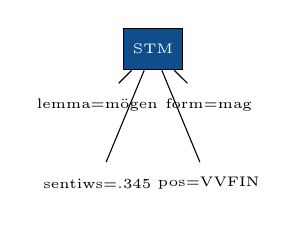
\begin{tikzpicture}
              [auto=right,scale=0.6,
                every node/.style={rectangle,draw=none,font=\tiny,fill=none,minimum size=15pt},
                word/.style={draw=none,fill=none}]
              \node[draw,align=center,text=white,fill=dodgerblue4] (n0) {STM};
              \node (n1) [below left of=n0] {lemma=m\"ogen};
              \node (n2) [below right of=n0] {form=mag};
              \node (n3) [below of=n1] {sentiws=.345};
              \node (n4) [below of=n2] {pos=VVFIN};
              \foreach \from/\to in {n1/n0,n2/n0,n3/n0,n4/n0}
              \draw (\from) -- (\to);
            \end{tikzpicture}
          }

          \only<5>{
            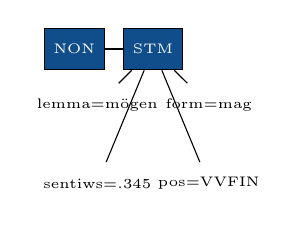
\begin{tikzpicture}
              [auto=right,scale=0.6,
                every node/.style={rectangle,draw=none,font=\tiny,fill=none,minimum size=15pt},
                word/.style={draw=none,fill=none}]
              \node[draw,align=center,text=white,fill=dodgerblue4] (n0) {STM};
              \node (n1) [below left of=n0] {lemma=m\"ogen};
              \node (n2) [below right of=n0] {form=mag};
              \node (n3) [below of=n1] {sentiws=.345};
              \node (n4) [below of=n2] {pos=VVFIN};
              \node (n5) [left of=n0,draw,text=white,fill=dodgerblue4] {NON};
              \foreach \from/\to in {n1/n0,n2/n0,n3/n0,n4/n0,n5/n0}
              \draw (\from) -- (\to);
            \end{tikzpicture}
          }

          \only<6>{
            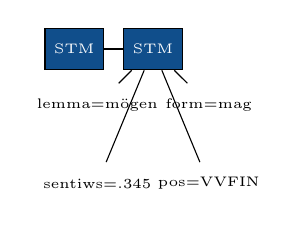
\begin{tikzpicture}
              [auto=right,scale=0.6,
                every node/.style={rectangle,draw=none,font=\tiny,fill=none,minimum size=15pt},
                word/.style={draw=none,fill=none}]
              \node[draw,align=center,text=white,fill=dodgerblue4] (n0) {STM};
              \node (n1) [below left of=n0] {lemma=m\"ogen};
              \node (n2) [below right of=n0] {form=mag};
              \node (n3) [below of=n1] {sentiws=.345};
              \node (n4) [below of=n2] {pos=VVFIN};
              \node (n5) [left of=n0,draw,text=white,fill=dodgerblue4] {STM};
              \foreach \from/\to in {n1/n0,n2/n0,n3/n0,n4/n0,n5/n0}
              \draw (\from) -- (\to);
            \end{tikzpicture}
          }

          \only<7>{
            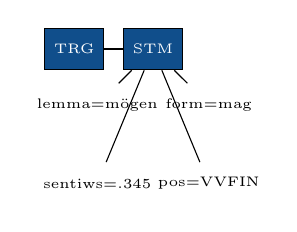
\begin{tikzpicture}
              [auto=right,scale=0.6,
                every node/.style={rectangle,draw=none,font=\tiny,fill=none,minimum size=15pt},
                word/.style={draw=none,fill=none}]
              \node[draw,align=center,text=white,fill=dodgerblue4] (n0) {STM};
              \node (n1) [below left of=n0] {lemma=m\"ogen};
              \node (n2) [below right of=n0] {form=mag};
              \node (n3) [below of=n1] {sentiws=.345};
              \node (n4) [below of=n2] {pos=VVFIN};
              \node (n5) [left of=n0,draw,text=white,fill=dodgerblue4] {TRG};
              \foreach \from/\to in {n1/n0,n2/n0,n3/n0,n4/n0,n5/n0}
              \draw (\from) -- (\to);
            \end{tikzpicture}
          }

          \only<8>{
            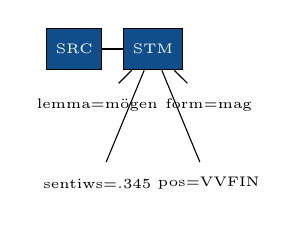
\begin{tikzpicture}
              [auto=right,scale=0.6,
                every node/.style={rectangle,draw=none,font=\tiny,fill=none,minimum size=15pt},
                word/.style={draw=none,fill=none}]
              \node[draw,align=center,text=white,fill=dodgerblue4] (n0) {STM};
              \node (n1) [below left of=n0] {lemma=m\"ogen};
              \node (n2) [below right of=n0] {form=mag};
              \node (n3) [below of=n1] {sentiws=.345};
              \node (n4) [below of=n2] {pos=VVFIN};
              \node (n5) [left of=n0,draw,text=white,fill=dodgerblue4] {SRC};
              \foreach \from/\to in {n1/n0,n2/n0,n3/n0,n4/n0,n5/n0}
              \draw (\from) -- (\to);
            \end{tikzpicture}
          }

          \only<9>{
            \begin{equation*}
              \alpha[t][j] = \sum_i{\alpha[t-1][i] * exp(f(y=j, y'=j))} * exp(\sum_k{\Theta_k * f_k(x = x_t, y = y_j)})
            \end{equation*}
          }
        \end{center}
      \end{minipage}
      \vspace*{\fill}
    \end{frame}

    \begin{frame}
        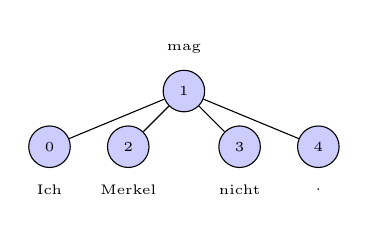
\begin{tikzpicture}
          [auto=left,scale=0.6,
            every node/.style={circle,draw,fill=blue!20,minimum size=15pt},
            every label/.style={shape=rectangle,draw=none,fill=none}]
          \node[align=center,label={\tiny mag}] (n0) {\tiny 1};
          \node (n2) [below left of=n0,label=below:{\tiny Merkel}] {\tiny 2};
          \node (n3) [below right of=n0,label=below:{\tiny nicht}] {\tiny 3};
          \node (n1) [left of=n2,label=below:{\tiny Ich}] {\tiny 0};
          \node (n4) [right of=n3,label=below:{\tiny .}] {\tiny 4};
          \foreach \from/\to in {n1/n0,n2/n0,n3/n0,n4/n0}
          \draw (\from) -- (\to);
        \end{tikzpicture}

        \vspace{1cm} \tiny $p(y|x) = \frac{exp\Big\{\sum_{k=1}^K\sum_{c \in
            Children(t)}{\lambda_k f_k (y_t, y_{c}, x_t)}\Big\}}{Z(x)}$
    \end{frame}

    \subsection{Data Change}
    \begin{frame}{Inter-annotator Agreement}
      \begin{table}
        \caption{\footnotesize Initial $\kappa$-Agreement for Sentiment
          Corpus}\centering
        \begin{tabular}{p{0.18\textwidth}*{5}{>{\centering\arraybackslash}p{0.13\textwidth}}}
          \hline\noalign{\smallskip}
          Element & Politics & Federal Election & General & Pope Election & Total\\
          \noalign{\smallskip} \hline
          Sentiment & 0.35 & 0.35 & 0.38 & 0.45 & 0.39\\
          Source & 0.39 & 0.27 & 0.28 & 0.41 & 0.37\\
          Target & 0.32 & 0.38 & 0.28 & 0.4 & 0.38\\
          Emo-expression & 0.64 & 0.57 & 0.72 & 0.68 & 0.64\\
          Diminisher & 0.67 & 0.44 & 0.8 & 0.0 & 0.37\\
          Intensifier & 0.46 & 0.48 & 0.73 & 0.21 & 0.52\\
          Negation & 0.44 & 0.1 & 0.21 & 0.36 & 0.28\\
          \noalign{\smallskip} \hline
        \end{tabular}
      \end{table}
    \end{frame}

    \begin{frame}{Annotation Improvement}
      \begin{table}
        \caption{\footnotesize $\kappa$-Agreement for Revised Sentiment
          Corpus} \centering
        \begin{tabular}{p{0.15\textwidth}*{5}{>{\centering\arraybackslash}p{0.13\textwidth}}}
          \hline\noalign{\smallskip}
          \multirow{2}{*}{Element} & %
          \multicolumn{2}{c}{\texttt{Politics}} & %
          \multicolumn{2}{c}{\texttt{Non-politics}} & \multirow{2}{*}{Gesamt}\\
          & Politik & Wahlen & Allgemein & Papstwahl\\
          \noalign{\smallskip} \hline
          Sentiment & 0.66 & 0.72 & 0.73 & 0.68 & 0.7\\
          Source & 0.72 & 0.77 & 0.71 & 0.69 & 0.73\\
          Target & 0.61 & 0.71 & 0.7 & 0.65 & 0.68\\
          Emo-expression & 0.83 & 0.84 & 0.88 & 0.86 & 0.86\\
          Diminisher & 0.67 & 0.64 & 0.62 & 0.18 & 0.53\\
          Intensifier & 0.51 & 0.62 & 0.6 & 0.37 & 0.56\\
          Negation & 0.55 & 0.58 & 0.6 & 0.66 & 0.6\\
          \noalign{\smallskip} \hline
        \end{tabular}
      \end{table}
    \end{frame}

    \begin{frame}{\insertsubsection}
      \begin{table}
        \tiny
        \caption{\scriptsize Classification results for automatic sentiment
          analysis.}  \centering
        \begin{tabular}{p{0.25\textwidth}*{3}{>{\centering\arraybackslash}p{0.15\textwidth}}}
          Classification Element & Precision & Recall & F-Measure\\\hline
          \multicolumn{4}{c}{\cellcolor{lightcyan4}Training Set}\\
            Sentiment & 99.23 \visiblealert{2}{98.51} & 86.27 \visiblealert{2}{85.63} &
            92.29  \visiblealert{2}{91.62}\\

            Source & 91.56 \visiblealert{2}{90.1} & 75.55 \visiblealert{2}{77.13} &
            82.78 \visiblealert{2}{83.11}\\

            Target & 95.99 \visiblealert{2}{97.08} & 75.69 \visiblealert{2}{80.09} &
            84.64 \visiblealert{2}{87.77}\\

          \hline\multicolumn{4}{c}{\cellcolor{lightcyan4}Test Set}\\
            Sentiment & 25 \visiblealert{2}{27.84} & 16.04 \visiblealert{2}{19.03} &
            19.55 \visiblealert{2}{22.61}\\

            Source & 47.06 \visiblealert{2}{31.25} & 25
            \visiblealert{2}{31.25} & 32.65 \visiblealert{2}{31.25}\\

            Target & 31.51 \visiblealert{2}{22.73} & 18.11
            \visiblealert{2}{20.47} & 23 \visiblealert{2}{21.54}\\
          \noalign{\smallskip} \hline
        \end{tabular}
      \end{table}
    \end{frame}


    \begin{frame}{\insertsubsection}
      \begin{table}
        \tiny
        \caption{\scriptsize Classification results for automatic sentiment
          analysis \visible<2->{(tree-structured CRF)}.}  \centering
        \begin{tabular}{p{0.25\textwidth}*{3}{>{\centering\arraybackslash}p{0.15\textwidth}}}
          Classification Element & Precision & Recall & F-Measure\\\hline
          \multicolumn{4}{c}{\cellcolor{lightcyan4}Training Set}\\
            Sentiment & 99.23 \visiblealert{2}{41.68} & 86.27 \visiblealert{2}{73.12} &
            92.29  \visiblealert{2}{53.1}\\

            Source & 91.56 \visiblealert{2}{44.13} & 75.55 \visiblealert{2}{67.54} &
            82.78 \visiblealert{2}{53.38}\\

            Target & 95.99 \visiblealert{2}{29.46} & 75.69 \visiblealert{2}{74.67} &
            84.64 \visiblealert{2}{42.25}\\

          \hline\multicolumn{4}{c}{\cellcolor{lightcyan4}Test Set}\\
            Sentiment & 25 \visiblealert{2}{24.86} & 16.04 \visiblealert{2}{27.46} &
            19.55 \visiblealert{2}{26.09}\\

            Source & 47.06 \visiblealert{2}{19.78} & 25
            \visiblealert{2}{18} & 32.65 \visiblealert{2}{18.85}\\

            Target & 31.51 \visiblealert{2}{18.24} & 18.11
            \visiblealert{2}{30.26} & 23 \visiblealert{2}{22.76}\\

          \noalign{\smallskip} \hline
        \end{tabular}
      \end{table}
    \end{frame}

    \subsection{Feature Change}

    \section{Current work}
    \subsection{RSTTool for Multilogues}
    \subsection{Preliminary Agreement Study}

    \nocite{Wiebe-94}
    \section*{Bibliography}
    \bibliography{bibliography}
    \bibliographystyle{plain}
    \end{document}
